%!TEX program=xelatex

% 碰到Windows版本提示Fandol字体,可以在命令行中以管理员权限执行:tlmgr update -self -all
%\documentclass[review]{cvpr}
\documentclass[final]{cvpr}

\usepackage[UTF8]{ctex}

%\usepackage{cvpr}
\usepackage{times}
\usepackage{epsfig}
\usepackage{graphicx}
\usepackage{amsmath}
\usepackage{amssymb}
\usepackage{subfigure}
\usepackage{overpic}
\setlength{\parindent}{2em}
\usepackage{enumitem}
\usepackage{indentfirst}
\setenumerate[1]{itemsep=0pt,partopsep=0pt,parsep=\parskip,topsep=5pt}
\setitemize[1]{itemsep=0pt,partopsep=0pt,parsep=\parskip,topsep=5pt}
\setdescription{itemsep=0pt,partopsep=0pt,parsep=\parskip,topsep=5pt}


\usepackage[pagebackref=true,breaklinks=true,colorlinks,bookmarks=false]{hyperref}


%\cvprfinalcopy % *** Uncomment this line for the final submission

\def\cvprPaperID{159} % *** Enter the CVPR Paper ID here
\def\confYear{CVPR 2020}
\def\httilde{\mbox{\tt\raisebox{-.5ex}{\symbol{126}}}}

\newcommand{\cmm}[1]{\textcolor[rgb]{0,0.6,0}{CMM: #1}}
\newcommand{\todo}[1]{{\textcolor{red}{\bf [#1]}}}
\newcommand{\alert}[1]{\textcolor[rgb]{.6,0,0}{#1}}

\newcommand{\IT}{IT\cite{98pami/Itti}}
\newcommand{\MZ}{MZ\cite{03ACMMM/Ma_Contrast-based}}
\newcommand{\GB}{GB\cite{conf/nips/HarelKP06}}
\newcommand{\SR}{SR\cite{07cvpr/hou_SpectralResidual}}
\newcommand{\FT}{FT\cite{09cvpr/Achanta_FTSaliency}}
\newcommand{\CA}{CA\cite{10cvpr/goferman_context}}
\newcommand{\LC}{LC\cite{06acmmm/ZhaiS_spatiotemporal}}
\newcommand{\AC}{AC\cite{08cvs/achanta_salient}}
\newcommand{\HC}{HC-maps }
\newcommand{\RC}{RC-maps }
\newcommand{\Lab}{$L^*a^*b^*$}
\newcommand{\mypara}[1]{\paragraph{#1.}}

\graphicspath{{figures/}}

% Pages are numbered in submission mode, and unnumbered in camera-ready
%\ifcvprfinal\pagestyle{empty}\fi
\setcounter{page}{409}
\begin{document}
% \begin{CJK*}{GBK}{song}

\renewcommand{\figref}[1]{图\ref{#1}}
\renewcommand{\tabref}[1]{表\ref{#1}}
\renewcommand{\equref}[1]{式\ref{#1}}
\renewcommand{\secref}[1]{第\ref{#1}节}
\def\abstract{\centerline{\large\bf 摘要} \vspace*{12pt} \it}

%%%%%%%%% TITLE

\title{基于欧拉方法的一维热传导数值求解问题}

\author{任立德\\
    南方科技大学\\
}

\maketitle
% \thispagestyle{empty}

%%%%%%%%% ABSTRACT
\begin{abstract}
	\setlength{\parindent}{2em}
本项目完成了对一维热传导方程的数值求解。在时间上采用了显式欧拉方法和隐式欧拉方法,在空间上采用了有限差分方法。通过调用PETSC完成对向量和矩阵对运算,通过调用MPI实现并行计算,通过HDF5文件保存数据。通过调整网格点大小和时间步大小对两种方法对稳定性和误差进行了分析。通过使用“-r”参数控制程序是否重启。通过使用“-np”调整CPU核数对代码并行效率进行分析。
\end{abstract}




%%%%%%%%% BODY TEXT %%%%%%%%%%%%%%%%%%%%%%%%%%%%%%%%%%%%%%%%
\section{理论推导}\label{sec:Introduction}
\setlength{\parindent}{2em}
已知一维热传导方程如下所示。
\begin{center}
		\begin{scriptsize}
\begin{equation}
	\setlength{\abovedisplayskip}{-5pt}
\rho c \frac{\partial u}{\partial t}-\kappa \frac{\partial^{2} u}{\partial x^{2}}=f
\end{equation}
\end{scriptsize}
\end{center}

根据有限差分法和显式欧拉方法可以得到如下公式。
\begin{center}
		\begin{scriptsize}
	\begin{equation}
			\setlength{\abovedisplayskip}{-5pt}
				\rho c \frac{u_{j}^{n+1}-u_{j}^{n}}{\Delta t}-\kappa \frac{u_{j-1}^{n}-2 u_{j}^{n}+u_{j+1}^{n}}{\Delta x^{2}}=f
	\end{equation}
\end{scriptsize}
\end{center}

经过推导得到第n+1个时间步,第j个网格点的$u_{j}^{n+1}$计算公式。
\begin{center}
	\begin{scriptsize}
	\begin{equation}
		\setlength{\abovedisplayskip}{-5pt}
		u_{i}^{n+1}=\frac{\kappa \Delta t}{\rho c \Delta x^{2}} u_{j-1}^{n}+\left(1-\frac{2\kappa \Delta t}{\rho c \Delta x^{2}}\right) u_{j}^{n} +\frac{\kappa \Delta t}{\rho c \Delta x^{2}} u_{j+1}^{n}+\frac{f \Delta t}{\rho c}
	\end{equation}
\end{scriptsize}
\end{center}

定义$\alpha=\frac{\kappa \Delta t}{\rho c \Delta x^{2}}$,则问题可以转换成三对角矩阵的求解。
\begin{center}
	\begin{scriptsize}
		\begin{equation}
			\setlength{\arraycolsep}{1pt}
			\setlength{\abovedisplayskip}{-5pt}
\left[\begin{array}{cccc}
	1-2 \alpha & \alpha& &  \\
	\alpha & 1-2\alpha & \alpha&  \\
	& \ddots & \ddots &  \\
	& &  \alpha& 1-2\alpha
\end{array}\right] \times\left[\begin{array}{c}
	u_{0}^{n} \\
	u_{1}^{n} \\
	\vdots \\
	u_{j}^{n}
\end{array}\right]+\left[\begin{array}{c}
	f_{0} \\
	f_{1} \\
	\vdots \\
	f_{j}
\end{array}\right]=\left[\begin{array}{c}
	u_{0}^{n+1} \\
	u_{1}^{n+1} \\
	\vdots \\
	u_{j}^{n+1}
\end{array}\right]
		\end{equation}
	\end{scriptsize}
\end{center}

同理根据有限差分法和隐式欧拉方法可以得到推导公式。
\begin{center}
	\begin{scriptsize}
		\begin{equation}
			\setlength{\abovedisplayskip}{-5pt}
-\frac{\kappa \Delta t}{\rho c \Delta x^{2}} u_{j-1}^{n+1}+\left(1+\frac{2\kappa \Delta t}{\rho c \Delta x^{2}}\right) u_{j}^{n+1}-\frac{\kappa \Delta t}{\rho c \Delta x^{2}} u_{j+1}^{n+1}=u_{j}^{n}+\frac{f \Delta t}{\rho c}
		\end{equation}
	\end{scriptsize}
\end{center}

隐式欧拉方法同样可以转换成三对角矩阵进行求解。
\begin{center}
	\begin{scriptsize}
		\begin{equation}
			\setlength{\arraycolsep}{1pt}
			\setlength{\abovedisplayskip}{-5pt}
\left[\begin{array}{cccc}
	1+2 \alpha & -\alpha & &  \\
	-\alpha & 1+2 \alpha & -\alpha &  \\
	& \ddots & \ddots & \\
	&  & -\alpha & 1+2\alpha
\end{array}\right] \times\left[\begin{array}{c}
	u_{0}^{n+1} \\
	u_{1}^{n+1} \\
	\vdots \\
	u_{j}^{n+1}
\end{array}\right]=\left[\begin{array}{c}
	u_{0}^{n} \\
	u_{1}^{n} \\
	\vdots \\
	u_{j}^{n}
\end{array}\right]+\left[\begin{array}{c}
	f_{0} \\
	f_{1} \\
	\vdots \\
	f_{j}
\end{array}\right]
		\end{equation}
	\end{scriptsize}
\end{center}

为了验证计算过程是否正确,还需要精确解作为参考。当$\frac{\partial u}{\partial t}=0$时,系统温度不随时间变化,可以看作稳定状态。即有如下公式。
\begin{center}
	\begin{scriptsize}
		\begin{equation}
			\setlength{\abovedisplayskip}{-5pt}
-\kappa \frac{\partial^{2} u}{\partial x^{2}}=\sin (l \pi x)
		\end{equation}
	\end{scriptsize}
\end{center}

根据边界条件求得微分方程的解析解为如下公式。
\begin{center}
	\begin{scriptsize}
		\begin{equation}
			\setlength{\abovedisplayskip}{-5pt}
			u(x)=\frac{1}{\kappa l^{2} \pi^{2}} \sin (l \pi x)
		\end{equation}
	\end{scriptsize}
\end{center}
%%%%%%%%%%%%%%%%%%%%%%%%%%%%%%%%%%%%%%%%%%%%%%%%%%%%%%%%%%%%%%%%%%%%%%%%%%%%%%%%%
\section{代码实现}
\label{sec:RelatedWorks}
项目将代码分成多个模块,每个模块解决特定问题。显式方法和隐式方法除了矩阵运算模块内部实现有所差别,其他模块基本相同。

在explicit.c中,模块一定义了与模型有关的多个常量参数,包括方程中的Rho、C、K等物理量以及GRID、TSTEP等控制网格点和迭代步长的参数。模块二定义了所需变量,包括计算时所需的向量和矩阵以及并行所需的rank变量和文件变量等。模块三对参数进行初始化,包括初始化petsc和mpi,以及读取“-r”参数。模块四计算并打印模型运算的重要信息,包括dx、dt等。模块五用于创建计算所需对向量和矩阵。模块六用于初始化三对角矩阵。模块七根据“-r”参数对初始条件进行初始化操作。当“-r”不存在时,表示程序无需重启,计算时直接从HDF5文件中获取数据。当“-r”不存在时,表示程序需要重启,默认时间t=0,重新计算各项数据。模块八用于迭代计算uj的值,从当前时间计算到初始设定的时间上限TEND,且迭代次数为10的整数倍时,将数据写入HDF5文件中,对数据进行更新。模块九用于关闭向量和矩阵,防止内存泄漏。

通过Makefile对代码进行编译,使用make explicit或make implicit即可生成相应对可执行文件,使用make clean可以清除所有生成的中间文件和可执行文件。使用explicit.LSF提交TaiYi脚本,通过“-r”和“-np”等参数对程序进行相应控制。程序执行完成或者强制中断后,均可生成对应对HDF5文件,可用于分析计算结果和代码性能以及用于继续计算。

完整代码及使用说明文档的github仓库链接为https://github.com/RenLide/HPC-project.git,TaiYi服务器中项目代码文件夹位置为/work/mae-renld/HPC/project。




%%%%%%%%%%%%%%%%%%%%%%%%%%%%%%%%%%%%%%%%%%%%%%%%%%%%%%%%%%
\section{计算结果分析}\label{sec:HC}
\subsection{精度分析}
选择精确解作为结果误差分析的基准。选择GRID=100,TSTEP=100000进行计算,此时CFL=0.2。计算结果如图(1)所示。可以看出显式欧拉方法的
\begin{figure*}[htbp]
	\centering
	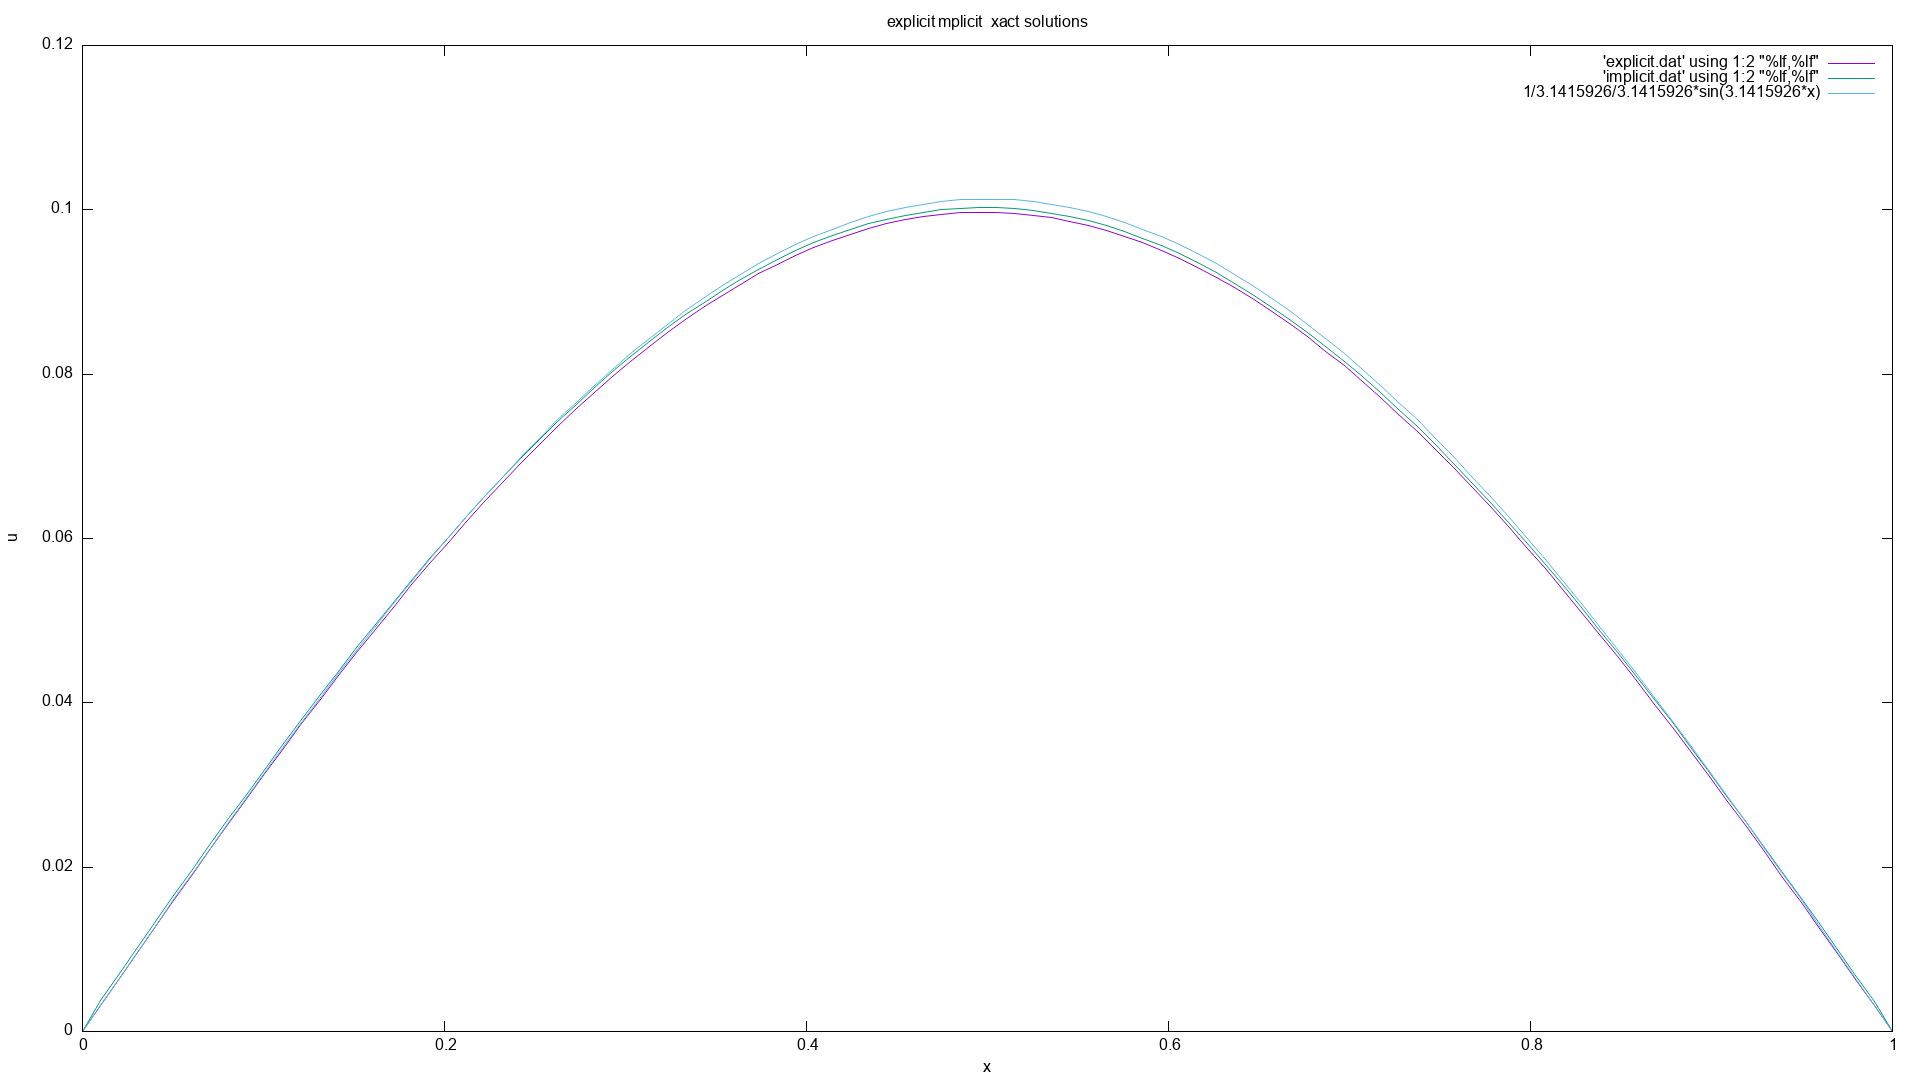
\includegraphics[scale=0.25]{./figures/solution_CFL0.2.png}
	\caption{solution CFL=0.2}
	\label{figure}
\end{figure*}



%%%%%%%%%%%%%%%%%%%%%%%%%%%%%%%%%%%%%%%%%%%%%%%
\subsection{稳定性分析}
对于显式欧拉方法,根据公式(3)进行冯诺依曼稳定性分析,可以得到如下公式。
\begin{center}
	\begin{scriptsize}
		\begin{equation}
			\begin{aligned}
				\setlength{\abovedisplayskip}{-5pt}
				\delta u_{j}^{n+1}=\alpha * \delta u_{j-1}^{n}+(1-2 \alpha) * \delta u_{j}^{n}+\alpha * \delta u_{j+1}^{n} 
			\end{aligned}
		\end{equation}
	\end{scriptsize}
\end{center}
即有如下近似公式。
\begin{center}
	\begin{scriptsize}
		\begin{equation}
			\setlength{\abovedisplayskip}{-5pt}
\delta u_{j}^{n+1} \sim e^{\delta n \Delta t} * e^{i(k * j \Delta x)}
		\end{equation}
	\end{scriptsize}
\end{center}
\begin{center}
	\begin{scriptsize}
		\begin{equation}
			\begin{aligned}
				\setlength{\abovedisplayskip}{-5pt}
				e^{\delta \Delta t}&=\alpha * e^{i k \Delta x}+(1-2 * \alpha)+\alpha * e^{-i k \Delta x}\\
				&=\alpha *\left(e^{i k \Delta x}+e^{-i k \Delta x}\right)+(1-2 * \alpha) \\
				&=1-2 \alpha+2 \alpha \cos (k \Delta x)
			\end{aligned}
		\end{equation}
	\end{scriptsize}
\end{center}
根据稳定条件可以计算出$\alpha$的取值范围,在代码中用CFL表示$\alpha$。
\begin{center}
	\begin{scriptsize}
		\begin{equation}
			\begin{aligned}
			\setlength{\abovedisplayskip}{-5pt}
			|1-2 \alpha+2 \alpha \cos (k \Delta x)| \leq 1&\Rightarrow-1 \leq 1-4 \alpha \leq 1  \\
			&\Rightarrow 0 \leq \alpha \leq \frac{1}{2}
			\end{aligned}
		\end{equation}
	\end{scriptsize}
\end{center}
在3.1精度分析中,取$\alpha=0.2$,显式与隐式欧拉方法均稳定。



%%%%%%%%%%%%%%%%%%%%%%%%%%%%%%%%%%%%%%%%%%%%%%


\mypara{颜色空间平滑}
虽然我们可以用颜色量化后的颜色直方图来高效计算颜色对比度,但量化本身可能会产生瑕疵。
因为一些相似的颜色可能被量化为不同的值。
为了减少这种随机性给显著性值计算带来的噪声,我们用平滑操作来改善每个颜色的显著性值。
每个颜色的显著性值被替换为相似颜色(用\Lab 距离测量)显著性值的加权平均。
这个过程实质上是颜色空间的一种平滑过程。
我们选择$m=n/4$个最近邻颜色来改善颜色$c$的显著性值,见公式:
\begin{equation}\label{equ:smoothing}
    S'(c) = \frac{1}{(m-1)T} \sum_{i=1}^{m} (T-D(c, c_i))S(c_i)
\end{equation}
其中 $T=\sum_{i=1}^{m} D(c, c_i)$ 为颜色 $c$和它的$m$ 个最近邻$c_i$之间的距离,
归一化因数由以下公式得到:
\begin{equation*}\label{equ:smoothingN}
    \sum_{i=1}^{m} (T-D(c, c_i))=(m-1)T.
\end{equation*}
我们用了一个线性变化平滑权值$(T-D(c, c_i))$来为在颜色特征空间中距离
$c$ 较近的颜色分配较大权值。
在我们的实验中,我们发现这种线性变化的权值比急剧下降的高斯权值的效果好。
\figref{fig:HCSmoothing}为颜色空间平滑后的效果,按显著性值降序排列。
注意到相似的直方图区间在平滑过后会非常接近,表明相似的颜色非常可能分配到相似的显著性值,
因此减少了量化的瑕疵(见 \figref{fig:plots})。


\mypara{实现细节}
为了将颜色空间量化为$12^3$种不同的颜色,我们统一将每个颜色的通道划分为12个等级。
虽然颜色量化在 RGB 颜色空间进行,
但为了颜色距离计算与人类感知更加符合,我们在 \Lab 颜色空间来测量颜色的距离。
我们并不直接在\Lab 颜色空间进行量化,因为并不是所有在区间$L^*\in[0, 100]$,
$a^*, b^*\in[-127,127]$中的颜色都对应真实的颜色。
实验结果表明,直接在 \Lab 空间量化得到效果并不好。
最佳结果是在 RGB 颜色空间量化,在\Lab 颜色空间测量距离得到的。




%%%%%%%%%%%%%%%%%%%%%%%%%%%%%%%%%%%%%%%%%%%%%%%%%%%%%%%%%%
\section{基于区域的对比度}




它与图像其它区域的颜色对比度来计算它的显著性值,
\begin{equation}\label{equ:regContrastSaliency}
    S(r_k) = \sum_{r_k \neq r_i} w(r_i)  D_r(r_k, r_i),
\end{equation}
其中$w(r_i)$为区域$r_i$的权值,$D_r(\cdot, \cdot)$为两个区域的颜色距离度量。
这里我们用 $r_i$里的像素数$w(r_i)$ 来强调大区域的颜色对比度。
两个区域$r_1$和$r_2$的颜色距离为:
\begin{equation}\label{equ:regContrast}
    D_r(r_1, r_2) = \sum_{i=1}^{n_1} \sum_{j=1}^{n_2} f(c_{1,i}) f(c_{2,j}) D(c_{1,i}, c_{2,j})
\end{equation}
其中$f(c_{k,i})$为第$i$个颜色$c_{k,i}$在第$k$个区域$r_k$的所有$n_k$种颜色中
出现的概率,$k=\{1,2\}$。
注意到我们使用区域的概率密度函数(即归一化的颜色直方图)中颜色出现概率作为权值,
以强调主要的颜色之间的区别。

因为每个区域只包含图像的直方图中很少数目的颜色,
所以为每个区域存储和计算常规矩阵形式的直方图是低效的。
我们用稀疏直方图以使得存储和计算过程更加高效。


%%%%%%%%%%%%%%%%%%%%%%%%%%%%%%%%%%%%%%%%%%%%%%%%%%%%%%%%%%

\begin{table*}
    \centering
    \begin{tabular}{l|c|c|c|c|c|c|c|c|c|c} \hline\hline
      方法  &  \IT   &  \MZ  &   \GB  &  \SR   &  \FT  &  \AC  &  \CA   & \LC   &  HC   &  RC   \\ \hline
      时间(秒) & 0.611  & 0.070 & 1.614  & 0.064  & 0.016 & 0.109 &  53.1  & 0.018 & 0.019 & 0.253 \\ \hline
      代码类型    & Matlab & C++   & Matlab & Matlab &  C++  &  C++  & Matlab &  C++  &  C++  &  C++  \\ \hline\hline
    \end{tabular}
    \caption{计算Achanta等人数据集\cite{09cvpr/Achanta_FTSaliency}中图像的平均用时。
        该数据集(参见我们主页)中大部分的图像分辨率为$400\times300$。
        这里所示的所有方法的时间是在一个拥有Dual Core 2.6 GHz
        CPU,2GB内存的机器上测得的。
    } \label{tab:TimeEfficency}
\end{table*}


\mypara{空间加权区域对比度 }
更进一步,通过在\equref{equ:regContrastSaliency}中引进空间权值,
我们将空间信息加入进来,来增加区域的空间影响效果。
近邻的区域增大影响,较远的区域减小影响。
特别地,对任意区域 $r_k$,基于空间加权区域对比度的显著性定义为:
\begin{equation}\label{equ:regContrastSpatial}
    S(r_k)=\sum_{r_k\neq r_i}\exp({-D_s(r_k,r_i)/\sigma_s^2})w(r_i) D_r(r_k, r_i)
\end{equation}
其中 $D_s(r_k, r_i)$ 为区域$r_k$ 和 $r_i$的空间距离,$\sigma_s$控制空间权值强度。
$\sigma_s$ 越大,空间权值的影响越小,导致较远区域的对比度会对当前区域显著性值做出较大的贡献。
两个区域的空间距离定义为两个区域重心的欧氏距离。在我们的试验中,$\sigma_s^2 = 0.4$,像素坐标归一化到$[0, 1]$区间。


%%%%%%%%%%%%%%%%%%%%%%%%%%%%%%%%%%%%%%%%%%%%%%%%%%%%%%%%%%%%%%%%%%%%%%
\section{实验比较}\label{sec:Experiment}


我们在Achanta等人提供的公开测试集\cite{09cvpr/Achanta_FTSaliency}上测试了我们的方法。
据我们所知,此测试集是此类数据最大的测试集,并且由人工精确标注了显著性区域。
我们将基于全局对比度的方法与其它$8$个当今最好的方法进行了比较。
仿照\cite{09cvpr/Achanta_FTSaliency},我们依据以下几个方面来选择其它方法来进行对比:
引用数(\IT ~和 \SR)、较新的方法(\GB, SR, \AC, \FT ~and \CA)、
多种类(IT 为生物驱动, \MZ~为纯计算, GB 为两者混合的, SR 在频域进行处理,
AC and FT 输出全分辨率显著性图),和我们方法最接近的(\LC)。


我们的方法和其它的方法在1000张图片上计算得到了显著性图。
\tabref{tab:TimeEfficency} 比较了每个方法的平均用时。
我们的方法HC和RC用C++实现,对于IT、GB、SR、FT和CA,我们引用了作者的实现。
由于找不到LC作者的源码,我们用C++来实现了此算法。
对于典型自然图片,HC 方法时间复杂度为 $O(N)$,对于实时应用已经非常高效。
相比之下,RC需要图像分割~\cite{04ijcv/felzenszwalb_efficient},
所以较慢,但它产生更好的效果。



为了全面的测试我们提出的方法的准确性,我们用了两种不同的客观比较方法进行了试验。
在第一个实验中,为了分割显著性物体并计算准确率召回率曲线,
我们参考\cite{09cvpr/Achanta_FTSaliency},用所有阈值分别将显著性图进行二值化。
在第二个试验中,我们用显著性图像初始化后迭代应用GrabCut方法
\cite{04tog/rother_grabcut}进行显著性物体分割。
我们还将得到的显著性图作为内容敏感的图像缩放和非真实感渲染的重要性权值。


%%%%%%%%%%%%%%%%%%%%%%%%%%%%%%%%%%%%%%%%%%%%%%%%%%%%%%%%%

\mypara{固定阈值的分割}
得到显著性物体的二值分割的最简单方法就是设定一个$T_f \in [0, 255]$的阈值。
为了可靠地比较多样的显著性检测方法高亮显著性物体的效果,
我们将阈值$T_f$设定为在$0$到$255$之间变化。\figref{fig:plots}为精确度召回率曲线结果。
我们还介绍了加入色彩空间平滑以及空间权值后的效果以及与其它方法的比较。
这些方法得到的显著性图的视觉直观比较在图~\ref{fig:cmp1vAll}
和图\ref{fig:VisualComparison}中。

正确率、召回率曲线清楚地展示出我们的方法优于其它的八种方法。
曲线的极限很有趣:在$T_f=0$处召回值最大,所有的像素被认为是前景,
所以所有的方法得到相同的正确值和召回值;这点的正确值为$0.2$,召回值为$1.0$。
这表明,在标注数据中,平均$20\%$的图像像素属于显著性区域。
曲线另一端,我们的方法的最小召回值比其它方法高,
因为我们的显著性图更加平滑,且包含更多显著性值为$255$的像素。


%%%%%%%%%%%%%%%%%%%%%%%%%%%%%%%%%%%%%%%%%%%%%
\mypara{显著性分割}
我们考虑将计算所得的显著性图像用于帮助显著物体分割。
在已有的工作中,显著性图已经被用于非监督物体分割:Ma和Zhang\cite{03ACMMM/Ma_Contrast-based}
通过在显著性图上进行模糊区域增长来找到矩形显著的区域。
Ko和Nam\cite{06josa/KoN_InterestSegmentation}在图像线段特征上训练支持向量机,
然后将这些区域聚类来提取显著性物体。
Han等人\cite{06TCSVT/han_unsupervised}用颜色、纹理和边缘特征建立马尔可夫
随机场模型,用显著性图的种子值来增长显著性物体区域。
最近,Achanta 等人~\cite{09cvpr/Achanta_FTSaliency}先通过mean-shift分割得到图像区域,
然后再图像区域内对显著性值进行平均,
再通过识别平均显著性值大于整个图像平均显著性值的2倍的图像区域来确定显著性区域。


在我们的方法中,我们迭代应用GrabCut \cite{04tog/rother_grabcut} 来改善二值化显著性
图像后得到的分割结果(见\figref{fig:AttCutSteps})。
传统的GrabCut方法是由人工选中矩形区域来进行初始化操作,
而我们用一个固定阈值二值化后的显著性图来得到显著性分割,
并用这个显著性分割来自动地进行GrabCut初始化。
这个阈值的我们经验性的选择固定阈值实验中与$95\%$召回率对应的阈值。


初始化之后,我们迭代运行GrabCut来改进显著性分割结果(在我们的实验中最多迭代 $4$ 次)。
在每一次迭代后,我们用膨胀和腐蚀操作来得到新的Trimap以进行下一次迭代。
如\figref{fig:AttCutSteps}所示,膨胀后仍然落在外面的区域设置成背景,
在腐蚀区域内的设置成前景,其余的区域为Trimap中的未知。
Grubcut本身是用高斯混合模型和Grapcut进行迭代,来改善每一步的区域分割效果,
靠近初始显著性物体区域的部分成为显著性物体的几率更大。
因此,我们的新的初始化方法可以使GrabCut包含显著性区域附近的显著性区域,
并根据颜色特征的差异排除非显著性区域。
在算法实现中,我们设置了狭窄的图像边界区域(15像素宽)作为背景来提高边界区域的收敛速度。


\figref{fig:AttCutSteps}展示了我们显著性分割算法的两个实例。
在旗子的例子中,不需要的区域被正确地排除;
在花朵的例子中,我们的方法扩展了初始显著性区域并收敛得到了精确的分割结果。
为了保持一致性,我们用召回率$95\%$的阈值对显著性图像进行二值化(见\figref{fig:plots})。
我们在基准数据集~\cite{09cvpr/Achanta_FTSaliency}上比较了平均正确率,召回率以及
$F$-测量,其中$F$-测量定义为:
\begin{equation}\label{equ:FMeasure}
    F_{\beta}= \frac{(1+\beta^2)Precision \times
        Recall}{\beta^2 \times Precision + Recall}.
\end{equation}

和Achanta等人\cite{09cvpr/Achanta_FTSaliency}一样,
我们用$\beta^2=0.3$来使正确率的权重高于召回率。
可以从比较结果(见\figref{fig:plots}-右和\figref{fig:cutCmp})中看出,
用我们的 RC 和 HC 显著性图来进行分割明显优于其它方法。
和当今最好的方法相比(正确率=$75\%$, 召回率=$83\%$),我们方法的结果更精确
(正确率=$90\%$, 召回率=$90\%$)。
(我们的演示程序可以从项目主页中得到。)


%%%%%%%%%%%%%%%%%%%%%%%%%%%%%%%%%%%%%%%%%%%%%%%%%%%%



\mypara{基于内容感知的图像缩放}
在内容敏感的图像缩放中,显著性图像经常用来指定图像的相对重要区域
(见~\cite{09_image_resize})。
我们用提取出的显著性图像进行了图像缩放实验。
实验中采用了Zhang等人提出的\cite{09cgf/ZhangC}内容敏感图像缩放方法
\footnote{我们采用作者公开的代码}。
该方法通过变形能量将变形分配到相对非显著性区域,同时保持全局和局部的图像特征。
\figref{fig:Resizing}比较了用\RC 和\CA 显著性图像得到的图像缩放结果。
显著性物体区域的显著性值是成片光滑的,这点对于基于能量的缩放非常重要,
因此我们的 RC 显著性图产生更好的缩放结果。
CA显著性图像在物体的边界有更高的显著性值,但这并不适于图像缩放等应用,
这些应用要求整个显著性物体一致的被突出。


%%%%%%%%%%%%%%%%%%%%%%%%%%%%%%%%%%%%%%%%%%%%%%%%%
\mypara{非真实感渲染}
艺术家们经常对图像抽象并突出有意义的部分并掩盖非重要区域\cite{99/zeki_innerVision}。
受此现象启发,一系列用显著性值来进行非真实感渲染的方法产生,
并产生了有趣的结果~\cite{02tog/decarlo_stylization}。
我们将我们的方法和最近的杰出的显著性检测方法~\cite{09cvpr/Achanta_FTSaliency}用在NPR
技术\cite{10pg/Huang_Zhang}上进行了比较(见\figref{fig:NPR})。
我们的\RC 提供更好的掩模,这可以帮助NPR方法更好地保留重要图像部分以及区域边界的细节,
同时平滑其它部分。


%%%%%%%%%%%%%%%%%%%%%%%%%%%%%%%%%%%%%%%%%%%%%%%%%%%%







%%%%%%%%%%%%%%%%%%%%%%%%%%%%%%%%%%%%%%%%%%%%%%%%%

\section{总结与展望}\label{sec:Conclusion}
我们提出了基于全局对比度的显著性计算方法,即基于直方图对比度~(HC) 和基于空间信息增强的区域对比度~(RC)方法。
HC方法速度快,并且产生细节精确的结果,RC方法可以产生空间增强的高质量显著性图像,但与此同时具有相对较低的计算效率。
我们在国际上现有最大的公开数据集上测试了我们的方法,并与之前已有八种最好的其它方法进行了比较。
实验结果表明,我们提出的方法在正确率和召回率上都明显优于其它方法,并且简单而高效。

在未来的工作中,我们计划研究包含空间关系且保留详细细节的显著性图像的高效计算算法,
并且希望研究能够处理具有复杂纹理的背景图像的显著性检测算法,
以克服我们现有算法在处理这类情况中存在的缺陷。
最后,我们还希望显著性图像的检测过程中进一步考虑人脸、对称性等高级因素。
我们相信显著性图像可以应用于高效物体检测\cite{06TCSVT/han_unsupervised},
可靠图像分类,鲁棒的图像景物分析~\cite{journal/tog/ChengZMHH10},
并提高图像检索效果\cite{tog09/ChenCT_Sketch2Photo}。


\paragraph{致谢.} 本项目受到了国家973计划(2011CB302205), 国家863计划(2009AA01Z327),
国家自然科学基金(U0735001),以及国家核高基计划(2011ZX01042-001-002)的支持.
程明明的工作受到了Google PhD fellowship, IBM PhD fellowship, 以及教育部博士研究生学术新人奖的资助。

{\small
\bibliographystyle{ieee}
\bibliography{Saliency}
}

% \end{CJK*}
\end{document}
